%Adapted from:
%https://tex.stackexchange.com/questions/364824/drawing-tree-like-symbols

\usepackage{tikz}
\usetikzlibrary{arrows,calc,positioning}

\makeatletter
\newcommand\RSloop{\@ifnextchar\bgroup\RSloopa\RSloopb}
\makeatother
\newcommand\RSloopa[1]{\bgroup\RSloop#1\relax\egroup\RSloop}
\newcommand\RSloopb[1]%
  {\ifx\relax#1%
   \else
     \ifcsname RS:#1\endcsname
       \csname RS:#1\endcsname
     \else
       \GenericError{(RS)}{RS Error: operator #1 undefined}{}{}%
     \fi
   \expandafter\RSloop
   \fi
  }
\newcommand\X{0}
\newcommand\RS[1]%
  {\begin{tikzpicture}
     [every node/.style=
       {circle,draw,fill,minimum size=3pt,inner sep=0pt,outer sep=0pt},
      line cap=round
     ]
   \coordinate(\X) at (0,0);
   \RSloop{#1}\relax
   \end{tikzpicture}
  }

  
\newcommand\RSdef[1]{\expandafter\def\csname RS:#1\endcsname}
\newlength\RSu
\RSu=2ex
\RSdef{n}{\draw (\X) node{};}
\RSdef{i}{\draw (\X) node{} -- + (90:\RSu) node{};}
\RSdef{d}{\draw[dashed] (\X) node{} -- + (90:\RSu) node{};}
\RSdef{l}{\draw (\X) node{} -- +(135:\RSu) node{};}
\RSdef{r}{\draw (\X) node{} -- +(45:\RSu) node{};}
\RSdef{I}{\draw (\X) node{} -- +(90:\RSu) coordinate(\X I);\edef\X{\X I}}
\RSdef{L}{\draw (\X) node{} -- +(135:\RSu) coordinate(\X L);\edef\X{\X L}}
\RSdef{R}{\draw (\X) node{} -- +(45:\RSu) coordinate(\X R);\edef\X{\X R}}

\RSdef{t}<1>{\draw (\X) node{};}


\newcommand{\treeOne}{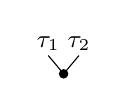
\begin{tikzpicture}
\coordinate (root) at (0, 0);
\filldraw (root) circle [radius=1.5pt];

\coordinate (left) at ($(root) + (130:2ex)$);
\node[] at ($(left) + (0,1ex)$) {\small $\tau_1$};

\coordinate (right) at ($(root) + (50:2ex)$);
\node[] at ($(right) + (0,1ex)$) {\small $\tau_2$};

\draw [thin] (left) to (root) to (right);
\end{tikzpicture}}

\newcommand{\treeTwo}{\begin{tikzpicture}
\coordinate (root) at (0, 0);
\filldraw (root) circle [radius=1.5pt];

\coordinate (top) at ($(root) + (0,2ex)$);
\node[] at ($(top) + (0,1ex)$) {\small $\tau_1$};

\draw [thin] (root) to (top);
\end{tikzpicture}}

\newcommand{\treeThree}{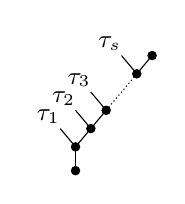
\begin{tikzpicture}
\coordinate (root) at (0, 0);
\filldraw (root) circle [radius=1.5pt];

\coordinate (node1) at ($(root) + (0,2ex)$);
\filldraw (node1) circle [radius=1.5pt];
\draw [thin] (root) to (node1);

\coordinate (node2) at ($(node1) + (50:2ex)$);
\filldraw (node2) circle [radius=1.5pt];
\draw [thin] (node1) to (node2);

\coordinate (node3) at ($(node2) + (50:2ex)$);
\filldraw (node3) circle [radius=1.5pt];
\draw [thin] (node2) to (node3);

\coordinate (node4) at ($(node3) + (50:4ex)$);
\filldraw (node4) circle [radius=1.5pt];
\draw [densely dotted] (node3) to (node4);

\coordinate (node5) at ($(node4) + (50:2ex)$);
\filldraw (node5) circle [radius=1.5pt];
\draw [thin] (node4) to (node5);

%labels
\coordinate (node11) at ($(node1) + (130:2ex)$);
\draw [thin] (node1) to (node11);
\node[] at ($(node11) + (-1ex,1ex)$) {\small $\tau_1$};

\coordinate (node21) at ($(node2) + (130:2ex)$);
\draw [thin] (node2) to (node21);
\node[] at ($(node21) + (-1ex,1ex)$) {\small $\tau_2$};

\coordinate (node31) at ($(node3) + (130:2ex)$);
\draw [thin] (node3) to (node31);
\node[] at ($(node31) + (-1ex,1ex)$) {\small $\tau_3$};

\coordinate (node41) at ($(node4) + (130:2ex)$);
\draw [thin] (node4) to (node41);
\node[] at ($(node41) + (-1ex,1ex)$) {\small $\tau_s$};

\end{tikzpicture}}

\newcommand{\commonRootTree}{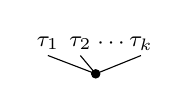
\begin{tikzpicture}
        \coordinate (root) at (0, 0);
        \filldraw (root) circle [radius=1.5pt];
        
        \coordinate (n1) at ($(root) + (159:4.3ex)$);
        \node[] at ($(n1) + (0,1ex)$) {\footnotesize $\tau_1$};
        
        \coordinate (n2) at ($(root) + (130:2ex)$);
        \node[] at ($(n2) + (0,1ex)$) {\footnotesize $\tau_2$};

        \coordinate (n3) at ($(root) + (50:2ex)$);
        \node[] at ($(n3) + (0,1ex)$) {\footnotesize $\cdots$};

        \coordinate (n4) at ($(root) + (22:4.1ex)$);
        \node[] at ($(n4) + (0,1ex)$) {\footnotesize $\tau_k$};
        
        \draw [thin] (n1) to (root);
        \draw [thin] (n2) to (root);
        \draw [thin] (n4) to (root);
    \end{tikzpicture}}


\newcommand{\treeFour}{
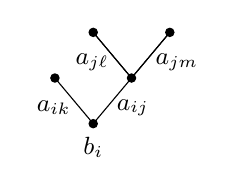
\begin{tikzpicture}
\coordinate (root) at (0, 0);
\filldraw (root) circle [radius=1.5pt];

\coordinate (left) at ($(root) + (130:5ex)$);
\filldraw (left) circle [radius=1.5pt];

\coordinate (right) at ($(root) + (50:5ex)$);
\filldraw (right) circle [radius=1.5pt];

\coordinate (rl) at ($(right) + (130:5ex)$);
\filldraw (rl) circle [radius=1.5pt];

\coordinate (rr) at ($(right) + (50:5ex)$);
\filldraw (rr) circle [radius=1.5pt];

\draw [thin] (left) to (root) to (right);
\draw [thin] (rl) to (right) to (rr);
\draw [thin] (rl) to (right) to (rr);

\node[] at ($(root) + (0ex,-2ex)$) {\small $b_i$};
\node[] at ($(left) + (-0.1ex,-2.5ex)$) {\small $a_{ik}$};
\node[] at ($(right) + (0.1ex,-2.5ex)$) {\small $a_{ij}$};
\node[] at ($(rl) + (-0.1ex,-2.5ex)$) {\small $a_{j\ell}$};
\node[] at ($(rr) + (0.6ex,-2.5ex)$) {\small $a_{jm}$};
\end{tikzpicture}}


\newcommand{\treeFive}{
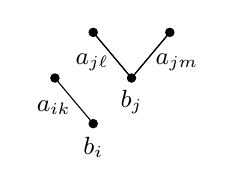
\begin{tikzpicture}
\coordinate (root) at (0, 0);
\filldraw (root) circle [radius=1.5pt];

\coordinate (left) at ($(root) + (130:5ex)$);
\filldraw (left) circle [radius=1.5pt];

\coordinate (right) at ($(root) + (50:5ex)$);
\filldraw (right) circle [radius=1.5pt];

\coordinate (rl) at ($(right) + (130:5ex)$);
\filldraw (rl) circle [radius=1.5pt];

\coordinate (rr) at ($(right) + (50:5ex)$);
\filldraw (rr) circle [radius=1.5pt];

\draw [thin] (left) to (root);
\draw [thin] (rl) to (right) to (rr);
\draw [thin] (rl) to (right) to (rr);

\node[] at ($(root) + (0ex,-2ex)$) {\small $b_i$};
\node[] at ($(left) + (-0.1ex,-2.5ex)$) {\small $a_{ik}$};
\node[] at ($(right) + (0ex,-2ex)$) {\small $b_j$};
\node[] at ($(rl) + (-0.1ex,-2.5ex)$) {\small $a_{j\ell}$};
\node[] at ($(rr) + (0.6ex,-2.5ex)$) {\small $a_{jm}$};
\end{tikzpicture}}



\newcommand{\treeSix}{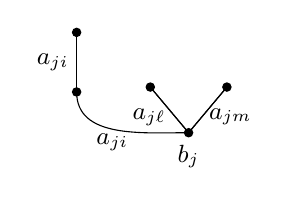
\begin{tikzpicture}

\coordinate (right) at (0, 0);
\filldraw (right) circle [radius=1.5pt];

\coordinate (rl) at ($(right) + (130:5ex)$);
\filldraw (rl) circle [radius=1.5pt];

\coordinate (rr) at ($(right) + (50:5ex)$);
\filldraw (rr) circle [radius=1.5pt];

% \draw [thin] (left) to (root);
\draw [thin] (rl) to (right) to (rr);
\draw [thin] (rl) to (right) to (rr);

\node[] at ($(right) + (0ex,-2ex)$) {\small $b_j$};
\node[] at ($(rl) + (-0.1ex,-2.5ex)$) {\small $a_{j\ell}$};
\node[] at ($(rr) + (0.3ex,-2.5ex)$) {\small $a_{jm}$};

\coordinate (newleft) at ($(right) + (160:10ex)$);
\filldraw (newleft) circle [radius=1.5pt];

\draw [thin] (right) to[out=180,in=270] (newleft);

\coordinate (ll) at ($(newleft) + (90:5ex)$);
\filldraw (ll) circle [radius=1.5pt];
\draw [thin] (newleft) to (ll);

\node[] at ($(newleft) + (3ex,-4.2ex)$) {\small $a_{ji}$};

\node[] at ($(ll) + (-2ex,-2.5ex)$) {\small $a_{ji}$};

\end{tikzpicture}}